 %!TEX root = ./template-skripsi.tex
%-------------------------------------------------------------------------------
%                            BAB II
%               KAJIAN TEORI
%-------------------------------------------------------------------------------

\chapter{KAJIAN PUSTAKA} 

\section{Pengertian \emph{Search Engine}}

\emph{Search engine} adalah sebuah mesin atau program yang mampu menampilkan banyak informasi yang relevan terkait dengan \textit{keyword} masukan pengguna. Sistem ini adalah sebuah sistem yang mengindeks, mengumpulkan segala informasi yang tersimpan dalam internet, menyaringnya berdasarkan \textit{keyword input}, dan menampilkan halaman \textit{website} terkait dengan perangkingan guna memudahkan dalam mendapatkan informasi.

Secara singkat, \textit{search engine} juga dapat disebut sebagai sebuah navigasi atau penunjuk dalam melakukan \textit{surfing} dalam dunia internet. Dengan memanfaatkan \textit{search engine}, kita dengan mudah akan mendapatkan informasi yang diperlukan dengan rekomendasi halaman yang paling terkenal berada dalam ranking paling atas.


\section{Sejarah \emph{Search Engine}}

Tahun 1990 adalah tahun pertama kemunculan \textit{search engine} untuk pertama kali dan diberi nama dengan \textit{Archive} atau \textit{Archie}. Dibangun oleh 3 mahasiswa Ilmu Komputer dari Universitas Mc Gill di Kanada bernama J.Peter Deutsch, Bill Heelan, dan Alan Emtage. \textit{Archie} lahir dari sebuah \textit{database} yang berisi \textit{file} dari ratusan sistem. Cara kerja \textit{Archie} tidak dengan mengindeks isi konten dari sebuah web, namun dengan cara menjangkau semua FTP dan membuat daftar \textit{file} untuk membuat indeks pencarian. Untuk dapat menggunakan \textit{Archie} dalam melakukan pencarian, diperlukan pengetahuan yang cukup tentang \textit{UNIX} karena \textit{Archie} dibangun menggunakan perintah-perintah \textit{UNIX} \citep{seymour2011history}.

Satu tahun setelah \textit{Archie} diluncurkan, muncullah \textit{Gopher} yang membawa dua  \textit{search engine} yang disebut \textit{Jughead} dan \textit{Veronice}. Dua program pencarian ini bekerja mirip \textit{Archie}, yakni mengumpulkan nama judul dan \textit{file} dan diindeks ke dalam \textit{Gopher}. Dibuat oleh Mark McCahill, \textit{Gopher} diharapkan dapat mencari, mengambil, dan menyebarkan \textit{file} melalui internet dengan tingkat penyimpanan informasi lebih kuat. Namun disayangkan, \textit{Gopher} memiliki beberapa fitur yang tidak mampu didukung oleh \textit{website} pada tahun 1991.

Pada tahun 1993, sebuah \textit{search engine} bernama \textit{Aliweb} telah rilis. Untuk melakukan pengindeksan, pengguna \textit{Aliweb} harus mendaftarkan situsnya ke \textit{Aliweb Server} \citep{seymour2011history}. Hal ini dikarenakan \textit{Aliweb} tidak mengindeks situs secara otomatis. Pada akhir tahun 1993, perilisan \textit{search engine} lain yang diberi nama \textit{Jumpstation} dilakukan. Dengan menggunakan \textit{web robot}, \textit{Jumpstation} mencari halaman web lalu mengindeksnya. Hal ini membuat \textit{Jumpstation} menjadi \textit{search engine} pertama yang memenuhi 3 fitur utama sebuah \textit{search engine} yakni \textit{searching}, \textit{indexing}, dan \textit{crawling}. Meski masih terbatas dalam pengindeksan, namun  \textit{Jumpstation} sanggup memberikan fasilitas pengindeksan \textit{headings} dan judul yang ditemukan di web.

Tahun 1994 pada bulan April, Brian Pinkerton dari Universitas Washington meluncurkan \textit{WebCrawler} yang menjadi \textit{search engine} pertama yang menawarkan pencarian teks secara lengkap di mana pengguna mampu mencari kata yang terdapat pada halaman web. Pengguna dapat memasukkan kata apapun yang mereka kira berhubungan dengan apa yang mereka cari dan \textit{Webcrawler} akan menampilkan setiap web yang memiliki kata tersebut. Hal ini di kemudian hari menjadi standar dari sebuah \textit{search engine}.

Setelah \textit{WebCrawler} bermunculan banyak \textit{search engine} serupa yang berusaha menyaingi demi popularitas. Beberapa \textit{search engine} yang bermunculan di antaranya adalah \textit{AltaVista}, \textit{Infoseek}, \textit{Inktomi}, dan \textit{Nocthern Light}. \textit{Yahoo!} dianggap salah satu yang terfavorit tetapi karena fungsi pencariannya hanya berada di direktori webnya, \textit{Yahoo!} membuat \textit{user} kurang nyaman karena teks tidak disalin dari \textit{website}.

Selanjutnya pada tahun 1995, \textit{AltaVista} menunjukkan kepopulerannya. Pengindeksan \textit{AltaVista} dibuat oleh Michael Burrows dan crawlernya dikerjakan oleh Louise Monier. \textit{Server} \textit{AltaVista} menjadi \textit{server} paling kuat yang mampu menangani jutaan hit dalam sehari, dan membuat \textit{AltaVista} menjadi \textit{search engine} paling cepat. Hal yang menyebabkan \textit{AltaVista} menjadi populer adalah adanya fitur yang mampu memunculkan informasi yang sesuai seperti yang dimasukkan dari \textit{user keyword}.

\textit{Ask Jeeves (Ask)} adalah \textit{search engine} yang dibuat oleh David Warthen dan Garrett Gruener dan didirikan tahun 1996 di Barkeley, California (Seymour et al., 2011). Ide awal \textit{Ask} muncul supaya memudahkan pengguna menemukan jawaban dari pertanyaan yang ditanyakan menggunakan bahasa yang umum digunakan. Saat ini \textit{Ask.com} masih tersedia dan terdapat fitur tambahan, yaitu dapat menerima pertanyaan matematika, kamus, dan pertanyaan konversi.

Dan pada tahun 1998, lahir satu \textit{search engine} yang di kemudian hari menjadi \textit{search engine} yang paling terkenal di seluruh negara. \textit{Google} diciptakan oleh Sergey Brin dan Larry Page yang merupakan mahasiswa Stanford California. Cara mereka untuk meningkatkan kualitas pencarian agar lebih akurat adalah dengan menambahkan fitur \textit{PageRank} yang di mana \textit{PageRank} adalah metode untuk menghitung peringkat setiap halaman web \citep{page1999pagerank}.

\textit{Google search engine} telah meminimalisir hasil penelusuran yang tidak berguna di hasil penelusuran teratas, sehingga memudahkan pengguna untuk mencari informasi yang ada di web. Mulai dari tahun 2000, \textit{Google search engine} menjadi terkenal hingga saat ini.

Di awal abad ke 20 tepatnya pada tanggal 18 Januari 2000, muncul \textit{search engine} bernama \textit{Baidu}. \textit{Baidu} berpusat di Beijing, RRC. \textit{Baidu} merupakan \textit{search engine} untuk \textit{website}, \textit{file audio} dan gambar berbahasa Cina dan Jepang. \textit{Baidu} merupakan perusahaan Cina yang masuk dalam indeks NASDAQ-100 pertama kali. Robin Li dan Eric Xu merupakan pendiri perusahaan \textit{Baidu}.

\textit{MSN search} diluncurkan pertama kali oleh Microsoft pada tahun 1998, menggunakan \textit{Inktomi} sebagai hasil penelusurannya \citep{seymour2011history}. Microsoft memiliki \textit{web crawler} sendiri bernama \textit{msnbot}, dan perlahan memulai menciptakan teknologi \textit{search engine} sendiri di tahun 2004 yang bernama \textit{Bing}. Bing resmi muncul pada tahun 2009 di awal bulan Juni. Kemudian satu bulan lebih setelahnya tepatnya tanggal 29 Juli 2009, Microsoft dan Yahoo! membuat kesepakatan di mana teknologi search engine \textit{Bing} akan mendukung hasil pencarian \textit{Yahoo! search}.

\begin{figure}[H]
	\centering
	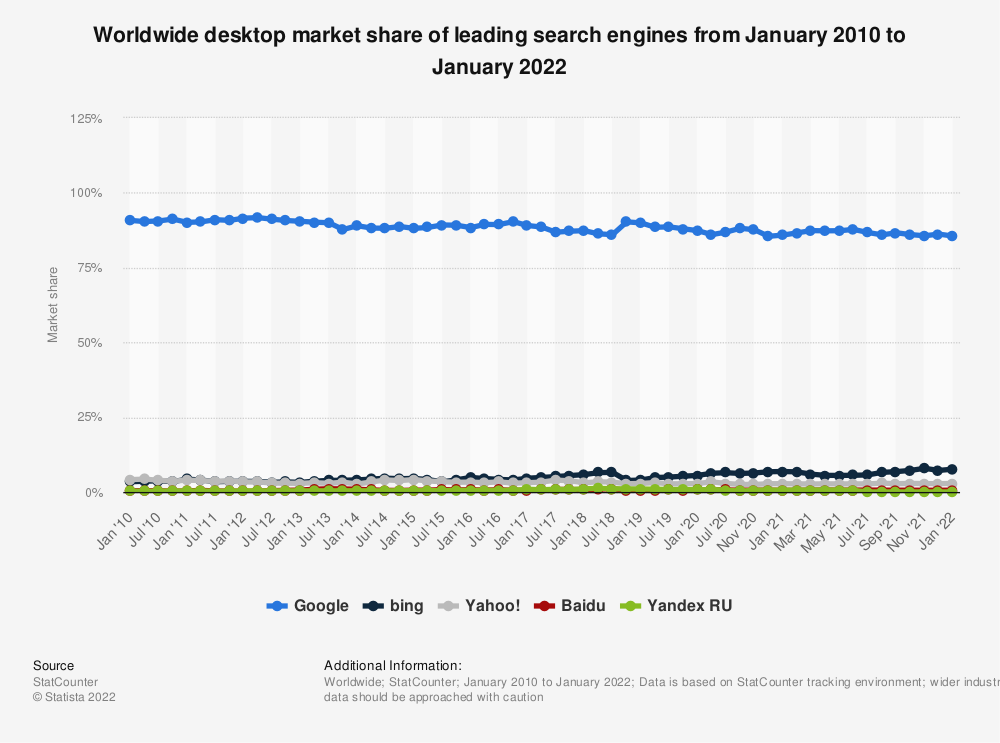
\includegraphics[keepaspectratio, width=12cm]{gambar/market_share_search_engine}
	\caption{\textit{Market share search engine} tahun 2010 hingga 2022 \citep{statista}}
	\label{gambar:market_share_search_engine}
\end{figure}

Berdasarkan data pada gambar \ref{gambar:market_share_search_engine}, \textit{search engine} yang paling banyak digunakan dari tahun 2010 hingga 2022 adalah \textit{Google}. Di peringkat kedua ada \textit{Yahoo} dan peringkat ketiga adalah \textit{Bing}. Selama 12 tahun \textit{Google} selalu berada di peringkat pertama dengan persentase di atas 85\%. Sedangkan \textit{Bing} dan \textit{Yahoo} pada bulan Januari 2022 memiliki persentase 7.61\% dan 2.85\%.

\section{Arsitektur \emph{Search Engine}}

Cara kerja \textit{search engine} adalah menyimpan semua informasi dari berbagai \textit{website}. Informasi dari halaman-halaman tersebut diekstrak menggunakan sebuah program yang disebut \emph{Web Crawler}, lalu konten di setiap halaman akan dianalisis untuk menentukan bagaimana halaman diindeks. Gambar \ref{gambar:google_architecture} merupakan \textit{High Level Google Architecture} \citep{brin1998anatomy}.

\begin{figure}[H]
	\centering
	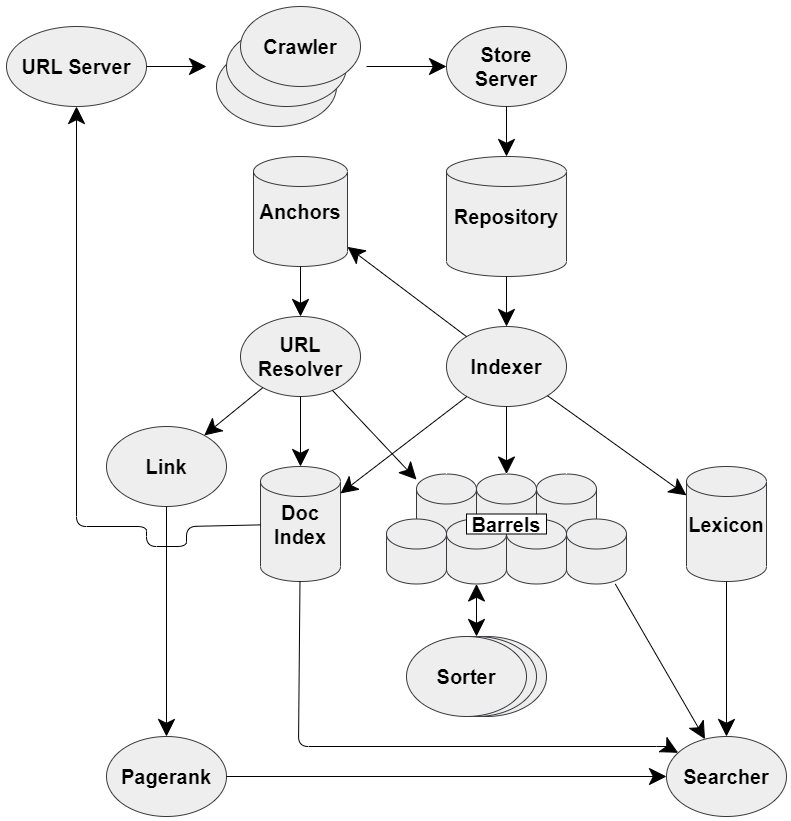
\includegraphics[keepaspectratio, width=10cm]{gambar/google_architecture}
	\caption{\emph{High Level Google Architecture} \citep{brin1998anatomy}}
	\label{gambar:google_architecture}
\end{figure}

Dari gambar \ref{gambar:google_architecture} dapat dijelaskan secara berurutan sebagai berikut:
\begin{enumerate}
	\item \textit{Server} mengirimkan \textit{URL} untuk dikumpulkan oleh crawler.
	\item Pengunduhan halaman \textit{dari URL tersebut} dijalankan oleh beberapa \textit{crawler}.
	\item Halaman web yang telah diunduh atau diekstrak dikirim ke \textit{store server}.
	\item Dari \textit{store server} berpindah untuk disimpan ke dalam \textit{repository} di mana setiap halaman web memiliki sebuah ID yang disebut \textit{docID}.
	\item Bagian \textit{indexer} dan \textit{sorter} melakukan pengindeksan.
	\item Setiap dokumennya dirubah menjadi sekumpulan kata yang disebut \textit{hits}.
	\item \textit{Indexer} menyalurkan \textit{hits} ke dalam satu set \textit{barrels} dan membuat \textit{forward index} yang diurutkan sebagian.
	\item \textit{Indexer} menguraikan \textit{URL} di setiap halaman web yang tersimpan dan menyaring informasi untuk disimpan ke dalam \textit{anchor file}.
	\item \textit{URL resolver} mendeteksi isi \textit{ancor file} dan merubah \textit{URL} yang sebelumnya relatif menjadi absolut, serta merubahnya menjadi sebuah docID.
	\item Menaruh \textit{anchor text} ke \textit{forward index} terkait \textit{docID} yang telah ditunjukkan \textit{anchor}.
	\item Membuat \textit{database} berisi link yang berpasangan dengan \textit{docID} untuk penghitungan \textit{PageRank}.
	\item \textit{Sorter} mengambil \textit{barrels} yang diurutkan berdasarkan \textit{docID} dan \textit{wordID} untuk menghasilkan \textit{inverted index}.
	\item Program \textit{DumpLexicon} mengambil daftar wordID dan menghasilkan \textit{lexicon} baru untuk dipakai oleh \textit{searcher} bersama dengan lexicon yang dibuat \textit{indexer}.
	\item \textit{Searcher} dilakukan oleh \textit{web server} dan memakai \textit{lexicon} yang dibuat oleh \textit{DumpLexicon} bersama dengan \textit{inverted index} dan \textit{PageRank} untuk menjawab pertanyaan.
\end{enumerate}

Saat mengimplementasikan proses ini pada tahun 1998, Google membutuhkan waktu kurang lebih 9 hari untuk mengunduh data dari 26 juta halaman web, yang berarti prosesnya membutuhkan waktu sekitar 33,44 halaman per detik. Proses ini berjalan secara berulang untuk mendapatkan perubahan informasi atau data yang baru dari seluruh halaman web. Hampir seluruh proses diimplementasikan menggunakan bahasa \textit{C} atau \textit{C++}, sisanya seperti \textit{crawler} dan \textit{URL server} menggunakan bahasa \textit{Python}.

\section{\emph{Web Crawler}}

\emph{Web Crawler} adalah program yang mengambil halaman web, biasanya untuk digunakan oleh mesin pencari \citep{pinkerton1994finding}. Secara kasar, \emph{crawler} dimulai dari \emph{URL} halaman awal $P_{0}$. Kemudian \emph{crawler} merayap ke $P_{0}$, mengekstrak semua \emph{URL} yang terdapat di dalam $P_{0}$, dan menambahkannya ke antrian \emph{URL} untuk dipindai. Setelah itu, \emph{crawler} mengambil \emph{URL} dari antrian (dengan urutan tertentu), dan mengulangi prosesnya \citep{cho1998efficient}.

\section{Arsitektur \emph{Web Crawler}}

\begin{figure}[H]
	\centering
	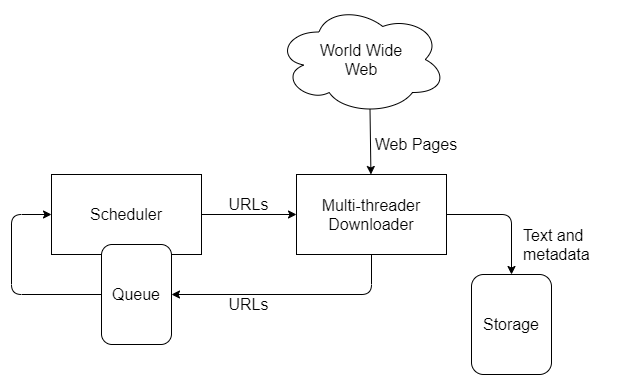
\includegraphics[keepaspectratio, width=12cm]{gambar/Arsitektur_Webcrawler}
	\caption{\emph{High Level Architecture of Web Crawler} \citep{castillo2005effective}}
	\label{gambar:architecture_webcrawler}
\end{figure}

\emph{Web crawler} adalah bagian penting dari \emph{search engine}. \emph{Crawler} membutuhkan strategi \emph{crawling} yang baik dan arsitektur yang sangat optimal. Desain sistem harus dioptimalkan untuk membentuk sistem berkinerja tinggi yang dapat mengunduh ratusan juta halaman selama beberapa minggu. \emph{High level architecture of Web crawler} ditunjukkan pada Gambar \ref{gambar:architecture_webcrawler}, membutuhkan \emph{scheduler} dan \emph{multi-threader downloader}. Dua struktur data utama adalah \emph{Web page} (\emph{text}) dan \emph{URL queue}.

\section{Algoritma \emph{Crawling}}

Secara umum, algoritma yang digunakan untuk \emph{crawling} menggunakan algoritma \emph{breadth first search}. Algoritma ini merupakan bentuk paling sederhana dari algoritma \textit{crawling}. Idenya adalah \textit{crawling} dimulai dari sebuah \emph{link}, kemudian terus mengikuti \emph{link} lain yang terhubung. Algoritma \emph{typical crawling model} dapat dilihat pada algoritma \ref{Typical_crawling_model} \citep{castillo2005effective}.

\begin{algorithm}[H]
	\caption{\emph{Typical Crawling Model} \citep{castillo2005effective}}
	\label{Typical_crawling_model}
	\begin{algorithmic}[1]
		\Require{$p_{1}, p_{2}, ..., p_{n}$ }{starting URLs}
		\State $Q = {p_{1}, p_{2}, ...,p_{n}}$, queue of URLs to visit.
		\State $V =  \emptyset$, visited URLs.
		\While{$Q\not=\emptyset$}
		\State Dequeue $p \in Q$, select $p$ according to some criteria.
		\State Do an asynchronous network fetch for $p$.
		\State $V = V\cup\{p\}$
		\State Parse $p$ to extract text and extract outgoing links
		\State $\Gamma^{+}(p) \gets$ pages pointed by p
		\For{each $p'\in\Gamma^{+}(p)$}
			\If{$p'\notin V \wedge p' \notin Q$}
			\State $Q = Q \cup \{p'\}$
			\EndIf
		\EndFor
		\EndWhile
	\end{algorithmic}
\end{algorithm}

Algoritma ini dimulai dengan mengumpulkan \textit{URL page} $p_{1}, p_{2},$ hingga $p_{n}$ ke dalam variabel $Q$. Kemudian, page tersebut dilakukan proses \textit{fetch} satu per satu dan mengambil teks serta \textit{outgoing link} dari \textit{page}. \textit{Outgoing link} yang didapat akan dimasukkan ke dalam variabel $Q$ jika link tersebut belum ada di variabel $Q$ dan belum masuk dalam proses \textit{fetch}. Proses ini akan berulang sampai \textit{page} pada variabel $Q$ kosong.

Karena sumber daya dan waktu yang terbatas, \textit{crawler} harus menentukan urutan \textit{URL} yang akan diproses terlebih dahulu. Algoritma \emph{modified similarity-based crawling} adalah algoritma untuk mengatasi masalah tersebut. \emph{Modified similarity-based crawling algorithm} dapat dilihat pada algoritma \ref{modified_sb_crawling} \citep{cho1998efficient}.

\begin{algorithm}[H]
	\caption{\emph{Modified similarity-based crawling} \citep{cho1998efficient}}
	\label{modified_sb_crawling}
	\begin{algorithmic}[1]
		\State enqueue(url\_queue, starting\_url);
		\While{(\textbf{not} empty(hot\_queue)) \textbf{and not} empty(url\_queue)}
			\State url = dequeue2(hot\_queue, url\_queue);
			\State page = crawl\_page(url);
			\If{[page contains 10 or more \emph{computer} in body or one \emph{computer} in title]}
				\State hot[url] = TRUE;
			\EndIf
			\State enqueue(crawled\_pages, (url, pages));
			\State url\_list = extract\_urls(page);
			\For{\textbf{each} u \textbf{in} url\_list}
			\State enqueue(links, (url, u));
			\If{[u \textbf{not in} url\_queue] \textbf{and}
				[u \textbf{not in} hot\_queue] \textbf{and}
				[(u,-) \textbf{not in} crawled\_pages]}
				\If{[u contains \emph{computer} in anchor or url]}
					\State enqueue(hot\_queue, u);
				\ElsIf{[distance\_from\_hotpage(u) < 3]}
					\State enqueue(hot\_queue, u);
				\Else
					\State enqueue(url\_queue, u);
				\EndIf
			\EndIf
			\State reorder\_queue(url\_queue);
			\State reorder\_queue(hot\_queue);
			\EndFor
		\EndWhile
	\end{algorithmic}
\end{algorithm}

Terdapat perbedaan pada algoritma \ref{Typical_crawling_model} \emph{typical crawling model} dan algoritma \ref{modified_sb_crawling} \emph{Modified similarity-based crawling}. Pada algoritma \ref{modified_sb_crawling} \emph{starting\_url} dimasukkan ke \emph{url\_queue}. Selain \emph{url\_queue}, ada juga \emph{hot\_queue}. \emph{hot\_queue} merupakan kumpulan \emph{URL hot page}. Suatu \emph{page} dikatakan \emph{hot}, karena memiliki salah satu dari kriteria berikut:

\begin{enumerate}
	\item Page yang berisi lebih dari 10 kata spesifik (dicontohkan sebagai kata "\emph{computer}") pada bagian \emph{body} atau 1 kata \emph{computer} di bagian \emph{title}.
	\item Kata spesifik (\emph{computer}) tersebut terdapat pada \emph{anchor} atau \emph{URL}.
	\item \emph{URL} yang memiliki hubungan dengan \emph{hot\_page}, masuk ke dalam kumpulan \emph{URL} di \emph{hot\_queue}, jika jaraknya kurang dari 3 \emph{link/node}.
\end{enumerate}

Kumpulan \textit{URL} baru yang didapat pada proses \textit{crawling} akan dimasukkan ke dalam \textit{hot\_queue} jika URL tersebut termasuk \textit{hot page}, jika tidak maka akan dimasukkan ke dalam \textit{url\_queue}. Lalu \textit{hot\_queue} dan \textit{url\_queue} akan diurutkan lagi pada fungsi \textit{reorder\_queue} dengan menggunakan \textit{backlink count}. \textit{URL} yang mempunyai nilai \textit{backlink count} tertinggi akan menempati urutan teratas dan akan diproses terlebih dahulu. Nilai \textit{backlink count} diperoleh dari banyaknya \textit{URL} yang ditempatkan pada \textit{URL} lain.

\section{\emph{Preprocessing Data}}

Setiap dokumen atau data seringkali memiliki struktur yang berubah-ubah atau tidak terstruktur. Oleh karena itu, diperlukan suatu proses yang dapat mengubah bentuk data yang sebelumnya tidak terstruktur menjadi data terstruktur. Proses konversi ini disebut \textit{text processing} \citep{feldman2007the}.

Data teks tersebut berisi banyak variasi dari mulai huruf hingga tanda baca. Variasi huruf harus konsisten, yaitu hanya menggunakan huruf besar saja atau huruf kecil saja. Selain itu, tanda baca juga perlu dihilangkan untuk mengurangi \textit{noise} selama pencarian informasi.

\textit{Preprocessing data} dilakukan agar data yang digunakan bebas noise, memiliki ukuran yang lebih kecil, dan lebih terorganisir sehingga dapat diproses lebih lanjut. Ada beberapa proses dalam tahap \textit{preprocessing data} yaitu \textit{case folding}, \textit{tokenizing}, \textit{stop word removal} dan \textit{stemming} seperti pada gambar \ref{gambar:preprocessing_data}.

\begin{figure}[H]
	\centering
	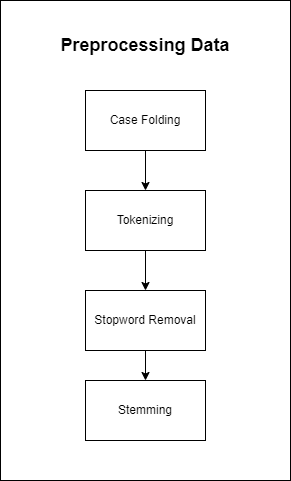
\includegraphics[keepaspectratio, width=6cm]{gambar/preprocessing_data}
	\caption{Tahapan \textit{preprocessing data}}
	\label{gambar:preprocessing_data}
\end{figure}

Proses pertama pada tahap \textit{preprocessing} adalah \textit{case folding}. Tujuan dari proses case folding adalah untuk menyamakan karakter pada data. Proses ini mengubah seluruh huruf pada data menjadi huruf kecil. Karakter-karakter huruf besar dari A sampai Z yang terdapat pada data diubah kedalam karakter huruf kecil a sampai z. Sedangkan karakter-karakter selain huruf seperti tanda baca dan angka akan dihilangkan dari data dan dianggap sebagai \textit{delimeter} atau batas pemisah \citep{manning2009anintroduction}.

Sebelum data teks dapat diproses lebih lanjut, data yang tadinya terdiri dari banyak kalimat harus dipecah menjadi kata-kata terpisah, yang mana proses ini disebut tokenization. Strategi umum yang dilakukan selama proses tokenization adalah memisahkan kata dengan \textit{whitespace} sebagai acuan pembatasnya dan menghilangkan tanda baca. Potongan-potongan kata yang sudah dihasilkan disebut dengan \textit{token}.

Tahap selanjutnya setelah \textit{tokenizing} adalah \textit{stop word removal} dan \textit{stemming}. \textit{Stop word removal} adalah pengambilan kata-kata penting dengan dari \textit{token} dengan cara membuang kata yang kurang penting atau tidak bermakna. Contoh \textit{stop word} dalam bahasa Indonesia dan akan dibuang dalam proses ini adalah "yang", "dan", "di", dll. Sedangkan \textit{stemming} adalah proses penghilangan imbuhan pada sebuah kata sehingga menjadi kata dasar.

\section{Pembobotan \emph{TF-IDF}}
Metode \textit{Term Frequency-Inverse Document Frequency} \textit{TF-IDF} adalah salah satu metode yang paling umum digunakan untuk menghitung bobot setiap kata dalam pencarian informasi. Cara ini juga dinilai efisien, sederhana dan memiliki hasil yang akurat.

\textit{TF-IDF} adalah metode pemberian bobot pada hubungan antara kata (\textit{word}) dan dokumen. \textit{TF-IDF} adalah ukuran statistik yang digunakan untuk mengevaluasi pentingnya sebuah kata dalam dokumen atau kumpulan kata. Frekuensi kata dalam dokumen tertentu menunjukkan pentingnya dalam dokumen. Frekuensi dokumen yang berisi kata tersebut menunjukkan seberapa umum kata tersebut. Jika sering muncul dalam satu dokumen, bobot kata lebih besar, dan jika muncul di banyak dokumen, bobot kata akan lebih kecil.

\textit{Term Frequency (TF)} menghitung berapa kali sebuah kata muncul dalam dokumen. Karena panjang setiap dokumen bisa berbeda, nilai \textit{TF} dibagi dengan panjang dokumen (jumlah kata dalam dokumen). Berikut rumus dari \textit{Term Frequency (TF)}:
\begin{equation}
tf_{t,d} = \frac{Number\>of\>times\>term\>t\>appears\>in\>a\>document}{Total\>number\>of\>terms\>in\>document}
\end{equation}

Di mana maksud dari pembilang pada persamaan di atas adalah jumlah kata t muncul dalam satu dokumen dan maksud dari penyebutnya adalah jumlah semua kata yang ada dalam satu dokumen tersebut.

Setelah menghitung \textit{Term Frequency (TF)}, selanjutnya adalah menghitung nilai \textit{Inverse Document Frequency (IDF)}, yang merupakan ukuran seberapa penting suatu kata. \textit{IDF} akan memberikan nilai pada kata-kata yang biasanya muncul sebagai kata yang kurang penting berdasarkan kemunculannya di seluruh dokumen. Semakin kecil nilai IDF, semakin tidak penting kata tersebut, dan sebaliknya. Berikut rumus dari \textit{Inverse Document Frequency (IDF)}:
\begin{equation}
idf_{t} = log (\frac{Total\>number\>of\>documents}{Number\>of\>documents\>with\>term\>t\>in\>it})
\end{equation}

Di mana maksud dari pembilang pada persamaan di atas adalah jumlah dokumen yang ada pada dataset dan maksud dari penyebutnya adalah jumlah dokumen pada dataset yang terdapat kata t di dalamnya.

Nilai idf dari kata yang kemunculannya jarang akan bernilai tinggi, sedangkan nilai idf dari kata yang kemunculannya sering nilainya akan cenderung rendah \citep{manning2009anintroduction}.

Setelah mempunyai nilai \textit{TF} dan \textit{IDF}, perhitungan bobot \textit{TF IDF} adalah hasil perkalian dari nilai \textit{TF} dan \textit{IDF}.
\begin{equation}
tfidf_{t,d} = tf_{t,d} \times idf_{t}
\end{equation}

\section{\emph{Google PageRank}}
Setiap kali melakukan pencarian di \textit{Google}, terdapat hasil \textit{website} yang muncul di halaman secara berurutan, sebagian itu adalah karena \textit{Google PageRank}. Sederhananya, \textit{PageRank} menganalisis jumlah tautan masuk ke setiap halaman di web, dan menetapkan setiap halaman sebuah peringkat yang ditentukan oleh peringkat setiap halaman yang menautkannya. \textit{PageRank} mengikuti model probabilistik dari seorang peselancar web, yang mengunjungi halaman tertentu, dan kemudian mengklik link di halaman itu secara acak. Intinya, peringkat setiap halaman mewakili kemungkinan bahwa setiap peselancar web akan mendarat di sana. Meskipun secara konseptual sederhana, \textit{PageRank} secara luas dianggap sebagai salah satu algoritma terpenting yang pernah ditemukan di industri teknologi.

Meskipun \textit{PageRank} secara populer dikaitkan dengan Larry Page dan Sergey Brin, pendiri \textit{Google}, versi awal masalah \textit{eigenvalue} dieksplorasi pada tahun 1976 oleh Gabriel Pinski dan Francis Narin dalam upaya mereka untuk menentukan peringkat jurnal ilmiah. Thomas Saaty mengeksplorasi masalah yang sama pada tahun 1977 dalam konsepnya tentang \textit{Analytic Heirarchy Process} yang menimbang keputusan, dan Bradley Love dan Steven Sloman menggunakannya pada tahun 1995 sebagai model kognitif untuk konsepnya juga.

Namun, baru pada tahun 1996 Larry Page dan Sergey Brin mengadopsi algoritma ini untuk digunakan dalam mesin pencari. Sebagai bagian dari proyek penelitian Stanford tentang penerapan mesin pencari jenis baru, Sergey Brin mengkonseptualisasikan gagasan untuk memeringkat halaman web dengan jumlah tautan yang mengarah ke sana. Makalah pertama mereka tentang masalah ini diterbitkan pada tahun 1998, yang mencakup prototipe awal mesin pencari Google, dan Page dan Brin juga mematenkan prosesnya (Universitas Stanford memegang paten, tetapi memberikan hak lisensi eksklusif kepada Google dengan imbalan 1,8 juta saham darinya). Sejak saat itu, algoritma ini tetap menjadi komponen integral dari mesin telusur \textit{Google} selama bertahun-tahun, meskipun ini bukan satu-satunya kriteria yang digunakan \textit{Google} untuk menentukan peringkat hasil penelusurannya.

Sebagai algoritma yang berlaku untuk \textit{graph} apa pun secara umum, \textit{PageRank} telah digunakan di banyak aplikasi lain selain mesin pencari, termasuk analisis jaringan jalan, ilmu saraf, bibliometrik, sastra, dan bahkan olahraga. Dalam industri teknologi, varian dari algoritma \textit{PageRank} tetap digunakan sampai sekarang; \textit{Twitter} menggunakannya untuk menyarankan pengguna untuk mengikuti, dan \textit{Facebook} mengimplementasikannya di belakang layar sebagai bagian dari algoritma teman yang disarankan.

Algoritma \textit{PageRank}, salah satu yang paling banyak digunakan terkait algoritma peringkat halaman, menyatakan bahwa jika suatu halaman memiliki \textit{link} penting ke sana, link ke halaman lain juga menjadi penting. Oleh karena itu, \textit{PageRank} memperhitungkan \textit{backlink} dan menyebarkan peringkat melalui tautan, yaitu sebuah halaman memiliki peringkat tinggi jika jumlah peringkat \textit{backlink}-nya tinggi. Gambar \ref{gambar:contoh_backlink} menunjukkan contoh dari \textit{backlink}: halaman A adalah \textit{backlink} halaman B dan halaman C sedangkan halaman B dan halaman C adalah \textit{backlink} dari halaman D.

\begin{figure}[H]
	\centering
	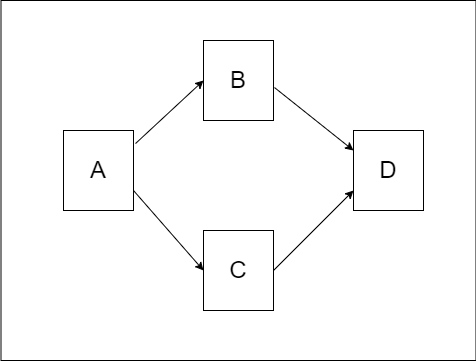
\includegraphics[keepaspectratio, width=8cm]{gambar/contoh_backlink}
	\caption{Contoh \textit{backlink}}
	\label{gambar:contoh_backlink}
\end{figure}

\subsection{\textit{Simplified PageRank}}
Versi \textit{PageRank} yang sedikit disederhanakan didefinisikan sebagai \citep{page1999pagerank}:

\begin{equation}
PR(u) = c \sum_{v \in B(u)}^{} \frac{PR(v)}{N_{v}}
\end{equation}

Di mana $u$ merepresentasikan halaman web. $B(u)$ adalah kumpulan halaman yang merujuk ke $u$. $PR(u)$ dan $PR(v)$ masing-masing merupakan skor peringkat halaman $u$ dan $v$. $N_{v}$ menunjukkan jumlah tautan keluar dari halaman $v$. Sedangkan $c$ adalah konstanta yang digunakan untuk normalisasi dan biasanya bernilai 0.85 namun dapat diubah sesuai keinginan.

Di \textit{PageRank}, skor peringkat halaman, $p$, dibagi rata di antara tautan keluarnya. Nilai yang ditetapkan ke tautan keluar halaman $p$ selanjutnya digunakan untuk menghitung peringkat halaman yang ditunjuk oleh halaman $p$. Skor peringkat halaman situs web dapat dihitung secara iteratif mulai dari halaman web mana pun. Dalam sebuah situs web, dua atau lebih halaman mungkin terhubung satu sama lain untuk membentuk satu lingkaran. Jika halaman ini tidak merujuk tetapi dirujuk oleh halaman web lain di luar \textit{loop}, mereka akan mengakumulasi peringkat tetapi tidak pernah mendistribusikan peringkat apa pun. Skenario ini disebut \textit{rank sink} \citep{page1999pagerank}.

\subsection{\textit{PageRank}}
Untuk mengatasi masalah \textit{rank sink}, diamati aktivitas pengguna. Sebuah fenomena ditemukan bahwa tidak semua pengguna mengikuti \textit{link} yang ada. Misalnya, setelah melihat halaman a, beberapa pengguna mungkin tidak memutuskan untuk mengikuti tautan yang ada tetapi langsung menuju ke halaman b, yang tidak langsung terhubung ke halaman a. Untuk tujuan ini, pengguna cukup mengetikkan \textit{URL} halaman b ke dalam kolom teks URL dan langsung melompat ke halaman b. Dalam hal ini, peringkat halaman b harus dipengaruhi oleh halaman a meskipun kedua halaman ini tidak terhubung langsung. Oleh karena itu, tidak ada \textit{rank sink} yang absolut. Berdasarkan pertimbangan fenomena tersebut di atas, PageRank yang original diterbitkan \citep{page1999pagerank}:

\begin{equation}
PR(u) = (1 - d) + d \sum_{v \in B(u)}^{} \frac{PR(v)}{N_{v}}
\end{equation}

Di mana $d$ merupakan \textit{damping factor} yang biasanya bernilai 0.85. Kita juga bisa menganggap $d$ sebagai probabilitas pengguna mengikuti tautan dan dapat menganggap $(1 - d)$ sebagai distribusi \textit{pagerank} dari halaman yang tidak terhubung secara langsung.

Untuk menguji kegunaan algoritma \textit{PageRank}, \textit{Google} menerapkannya pada mesin pencari \textit{Google}. Dalam percobaan, algoritma \textit{PageRank} bekerja secara efisien dan efektif karena nilai peringkat konvergen ke toleransi yang wajar dalam logaritma kasar $(log\>n)$ \citep{page1999pagerank}. Skor peringkat halaman web dibagi secara merata di atas halaman yang ditautkannya. Meskipun algoritma \textit{PageRank} berhasil digunakan di \textit{Google}, terdapat satu masalah yang masih ada: di web yang sebenarnya, beberapa tautan di halaman web mungkin lebih penting daripada yang lain \citep{xing2004weighted}.

\section{Metode Scrum}
Metode Scrum diciptakan oleh Jeff Sutherland dan tim pengembangnya pada awal 1990-an. Sutherland, Viktorov, Blount dan Puntikov menggambarkan Scrum sebagai “Proses pengembangan perangkat lunak \textit{Agile} yang dirancang untuk menambah energi, fokus, kejelasan, dan transparansi bagi tim proyek yang mengembangkan sistem perangkat lunak” \citep{sutherland2007}. Proses Scrum mematuhi prinsip-prinsip pendekatan \textit{Agile}. Prinsip pendekatan \textit{Agile} berfokus pada memuaskan pelanggan melalui pengiriman awal perangkat lunak yang berharga; membolehkan perubahan kebutuhan; kolaborasi antara pengembang dan pelaku bisnis; perangkat lunak yang berfungsi (sebagai ukuran kemajuan); menjaga desain tetap sederhana; dan secara berkala, membuat tim merenungkan bagaimana menjadi lebih efektif selama proses pengembangan.

Scrum menawarkan cara yang dapat disesuaikan untuk bekerja pada proyek yang berbeda yang memiliki berbagai persyaratan dan Scrum memiliki keunggulan seperti pemilihan persyaratan atau spesifikasi kebutuhan yang fleksibel untuk \textit{sprint} dan tidak ada prosedur khusus yang harus diikuti. Prinsipnya adalah bekerja secara iteratif hingga mencapai waktu yang ditentukan dan dapat memenuhi kebutuhan konsumen.

\section{Tim Scrum}
Tim Scrum setidaknya terdiri dari \textit{Product Owner}, \textit{Development Team} dan \textit{Scrum Master}. Tim Scrum adalah tim yang lintas fungsi, di mana anggotanya memiliki semua keterampilan yang diperlukan untuk melakukan pekerjaan tanpa bergantung pada orang lain di luar tim pada setiap \textit{Sprint}. Anggota tim Scrum juga mengatur diri mereka sendiri yang berarti secara internal mereka memutuskan siapa melakukan apa, kapan, dan bagaimana. Berikut merupakan anggota-anggota dari Tim Scrum.

\begin{enumerate}
	\item \textit{Product Owner}
	
	Pemilik produk (\textit{product owner}) adalah peran yang berfokus pada keberhasilan produk. Pemilik produk mencoba memaksimalkan nilai produk perangkat lunak bagi penggunanya. Oleh karena itu, pemilik produk bekerja secara kolaboratif dengan tim pengembangan dalam satu tim dan memberikan arahan pengembangan produk melalui visi produk mereka. Peran ini mengutamakan pekerjaan tim pengembang agar dapat diperoleh nilai terbaik dari produk perangkat lunak secara bertahap dan iteratif. 

Selain berkolaborasi dengan tim pengembangan, Pemilik produk membangun kemitraan aktif dengan para pemangku kepentingan. Pemangku kepentingan adalah siapa pun di luar tim yang tertarik pada keberhasilan produk perangkat lunak. Manajemen, pelanggan, dan sponsor produk, kita dapat menyebutnya sebagai pemangku kepentingan.

Pemilik produk adalah individu, bukan kelompok. Pemilik produk mewakili suara para pemangku kepentingan, mencari kesamaan di antara banyak kepentingan produk melalui komunikasi yang baik.

	\item \textit{Development Team}
	
	Tim pengembangan (\textit{development team}) adalah tim dengan berbagai peran yang diperlukan untuk membangun produk perangkat lunak. Beberapa peran khusus yang sering kita temui adalah \textit{software developer}, \textit{UI/UX designer}, dan \textit{quality assurance}. Peran-peran ini berkolaborasi setiap hari dalam tim pengembangan untuk membangun produk perangkat lunak sesuai dengan prioritas kerja yang disepakati dengan pemilik produk.

Di dalam Scrum, siapa pun yang termasuk dalam tim pengembangan disebut pengembang. Tidak ada peran khusus dalam tim pengembangan seperti yang didefinisikan oleh Scrum. Setiap orang adalah pengembang, dan siapa pun dapat melakukan apa saja untuk membangun perangkat lunak berkualitas tinggi. Membuat tim pengembangan lintas fungsi dan mengatur diri sendiri bukanlah tugas yang mudah. Ada proses yang membutuhkan waktu dan kesabaran untuk meningkatkan tim untuk mencapai level itu.

	\item \textit{Scrum Master}
	
	\textit{Scrum master} adalah peran yang berfokus pada keberhasilan implementasi proses perangkat lunak yang dihasilkan dari metode Scrum. \textit{Scrum master} memastikan aktivitas pengembangan dengan mengikuti proses Scrum. \textit{Scrum master} membantu pemilik produk dan tim pengembang bekerja sama dalam kerangka proses Scrum.

Sebagai pelatih, \textit{scrum master} melatih tim Scrum untuk menggunakan Scrum dengan tepat dalam lingkungan organisasi sehari-hari untuk mendapatkan manfaat terbaik dari Scrum. \textit{Scrum master} membantu semua orang di tim Scrum memahami tujuan dan manfaat Scrum untuk pengembangan produk perangkat lunak yang sukses.

Sebagai fasilitator, \textit{scrum master} menjadi fasilitator di tim Scrum selama pertemuan Scrum. \textit{Scrum master} mencari keputusan antara Pemilik Produk dan Tim Pengembang untuk memberikan perangkat lunak terbaik yang dihasilkan melalui musyawarah.

Sebagai agen perubahan, \textit{scrum master} membawa perubahan pada tim dan organisasi menuju implementasi proses Scrum yang lebih baik. Untuk organisasi baru, \textit{scrum master} memperkenalkan organisasi ke Scrum dan membantu organisasi mengadopsi Scrum. \textit{Scrum master} memandu proses perubahan dari proses perangkat lunak yang tidak terdefinisi ke proses Scrum.

\end{enumerate}

\section{Aktivitas-aktivitas Scrum (\textit{Scrum Events})}
Aktivitas-aktivitas pada Scrum dibuat untuk menciptakan kontinuitas dan mengurangi fase lain yang tidak terdaftar di Scrum. Terjadinya kegagalan dalam menerapkan salah satu dari tahapan ini akan mengurangi transparansi dan menghilangkan peluang untuk peninjauan dan perubahan. Aktivitas-aktivitas yang terdapat pada Scrum adalah sebagai berikut.
\begin{enumerate}
	\item \textit{Sprint}
	
	\textit{Sprint} merupakan tahap pengembangan perangkat lunak dengan durasi maksimum satu bulan dan memiliki durasi yang konsisten selama proses pengembangan produk. \textit{Sprint} baru akan langsung dimulai segera setelah \textit{Sprint} sebelumnya selesai. Sprint terdiri dari \textit{Sprint Planning}, \textit{Daily Scrum}, \textit{Sprint Review} dan \textit{Sprint Retrospective}.
	
	\item \textit{Sprint Planning}
	
	Pekerjaan yang dilakukan dalam \textit{Sprint} direncanakan dalam tahap \textit{Sprint Planning}. Rencana tersebut dibuat oleh semua anggota dalam tim Scrum. Untuk \textit{Sprint} yang berdurasi satu bulan, batas waktu \textit{Sprint Planning} maksimal 8 jam.
	
	\item \textit{Daily Scrum}
	
	\textit{Daily Scrum} adalah aktivitas yang berlangsung hingga 15 menit dan bertujuan agar tim pengembang dapat menyinkronkan pekerjaan mereka dan membuat rencana untuk 24 jam ke depan. Hal ini dilakukan dengan meninjau pekerjaan sejak tahap \textit{Daily Scrum} terakhir dan memperkirakan apa yang dapat dilakukan sebelum melanjutkan ke \textit{Daily Scrum} berikutnya.
	
	\item \textit{Sprint Review}
	
	\textit{Sprint Review} diadakan di akhir setiap \textit{Sprint} untuk meninjau iterasi dan merevisi \textit{Product Backlog} sesuai kebutuhan. Selama \textit{Sprint Review}, Tim Scrum dan pemangku kepentingan berkolaborasi untuk membahas pekerjaan yang telah dilakukan dalam \textit{Sprint} yang baru saja selesai. Berdasarkan hasil ini dan setiap perubahan pada \textit{Product Backlog} selama Sprint, peserta berkolaborasi untuk menentukan apa yang dapat dilakukan di \textit{Sprint} berikutnya untuk mengoptimalkan nilai produk. Pertemuan bersifat informal, bukan pertemuan status, dan pemaparan diharapkan dapat menghimpun masukan dan menumbuhkan semangat kerja sama.
	
	\item \textit{Sprint Retrospective}
	
	Sprint Retrospective adalah kesempatan bagi Tim Scrum untuk meninjau diri mereka masing-masing dan mengembangkan rencana untuk perbaikan di \textit{Sprint} berikutnya. \textit{Sprint Retrospective} dilakukan setelah \textit{Sprint Review} selesai dan sebelum \textit{Sprint Planning} berikutnya. Batas waktu maksimum tahap ini adalah 3 jam untuk \textit{Sprint} yang berdurasi satu bulan. Untuk \textit{Sprint} yang lebih pendek, batas waktunya biasanya lebih pendek. \textit{Scrum Master} memastikan bahwa langkah-langkah ini dilakukan dan semua anggota memahami tujuan mereka. \textit{Scrum Master} mendidik Tim Scrum untuk mengimplementasikannya dalam batas waktu yang telah ditentukan. \textit{Scrum Master} berpartisipasi sebagai mitra yang bertanggung jawab atas setiap proses yang terjadi saat Scrum terjadi.

\end{enumerate}

\section{Komponen Scrum}
Komponen Scrum mewakili pekerjaan atau nilai. Mereka dirancang untuk memaksimalkan transparansi informasi penting. Jadi setiap orang yang mengkajinya memiliki dasar adaptasi yang sama. Berikut merupakan komponen-komponen yang terdapat pada metode Scrum.
\begin{enumerate}
	\item \textit{Product Backlog}
	
	\textit{Product Backlog} adalah daftar apa yang dibutuhkan untuk meningkatkan produk. \textit{Item} dari \textit{Product Backlog} yang dapat dijalankan oleh Tim Scrum dalam sebuah \textit{Sprint} dianggap siap untuk diseleksi dalam aktivitas \textit{Sprint Planning}. Mereka biasanya mendapatkan transparansi ini setelah melakukan kegiatan revisi. Perbaikan \textit{Product Backlog} adalah operasi yang memecah dan mendefinisikan lebih lanjut \textit{item-item} Product Backlog menjadi \textit{item} yang lebih kecil dan lebih tepat. Menambahkan detail seperti deskripsi, urutan, dan ukuran diperlukan. Pengembang yang akan melakukan pekerjaan bertanggung jawab atas pengukuran. Pemilik produk dapat memengaruhi pengembang dengan membantu mereka memahami dan memilih.
	
	\item \textit{Sprint Backlog}
	
	\textit{Sprint Backlog} mencakup tujuan Sprint (mengapa), item \textit{Product Backlog} yang dipilih untuk \textit{Sprint} (apa), dan rencana yang layak untuk memberikan \textit{Increment} (bagaimana). \textit{Sprint Backlog} adalah rencana yang dibuat oleh pengembang. Ini adalah gambaran waktu nyata dari pekerjaan yang direncanakan pengembang selama \textit{Sprint} untuk mencapai tujuan \textit{Sprint}. Oleh karena itu, \textit{Sprint Backlog} diperbarui sepanjang \textit{Sprint} karena semakin banyak yang dipelajari. Ini harus cukup detail sehingga mereka dapat memeriksa seluruh kemajuan mereka di \textit{Daily Scrum}.
	
	\item \textit{Increment}
	
	Peningkatan (\textit{Increment}) adalah komponen yang dianggap sebagai batu loncatan untuk mencapai tujuan produk. Setiap peningkatan melengkapi semua tambahan sebelumnya dan diverifikasi secara menyeluruh untuk memastikan semua tambahan berfungsi secara maksimal. Beberapa penambahan dapat dilakukan di \textit{Sprint}. Total yang ditambahkan diberikan dalam diskusi \textit{Sprint}. Namun, Peningkatan dapat dikirim ke pemangku kepentingan sebelum \textit{Sprint} selesai. Diskusi \textit{Sprint} tidak boleh dianggap sebagai referensi untuk evaluasi. \citep{schwaber2020}
	
\end{enumerate}